\section{Hacia un Framework para la Comparación de Permisos}
\begin{frame}
 \begin{center}
  \LARGE Framework \\para la \\Comparación de Permisos
 \end{center}
\end{frame}
\begin{frame}
 \frametitle{Hacia un Framework para la Comparación de Permisos}
 \begin{block}{}
Se ha desarrollado un \textit{framework} para determinar empíricamente el alcance de los sistemas de permisos de ambas plataformas.
 \end{block}\pause
 \begin{columns}
  \begin{column}[]{.45\textwidth}
   \begin{exampleblock}{Objetivo I}
    {Se busca dejar en evidencia posibles vulnerabilidades presentes en los modelos de seguridad.}
   \end{exampleblock}
  \end{column}
  \begin{column}[]{.53\textwidth}\pause
   \begin{exampleblock}{Objetivo II}
    {Se intenta averiguar cuál es la cobertura del sistema de permisos respecto de los datos sensibles para la privacidad.}
   \end{exampleblock}
  \end{column}
 \end{columns}
\end{frame}
\begin{frame}
 \frametitle{Hacia un Framework para la Comparación de Permisos}
 \begin{columns}
  \begin{column}[]{.4\textwidth}
    \begin{figure}[hbtp]
     \centering
	 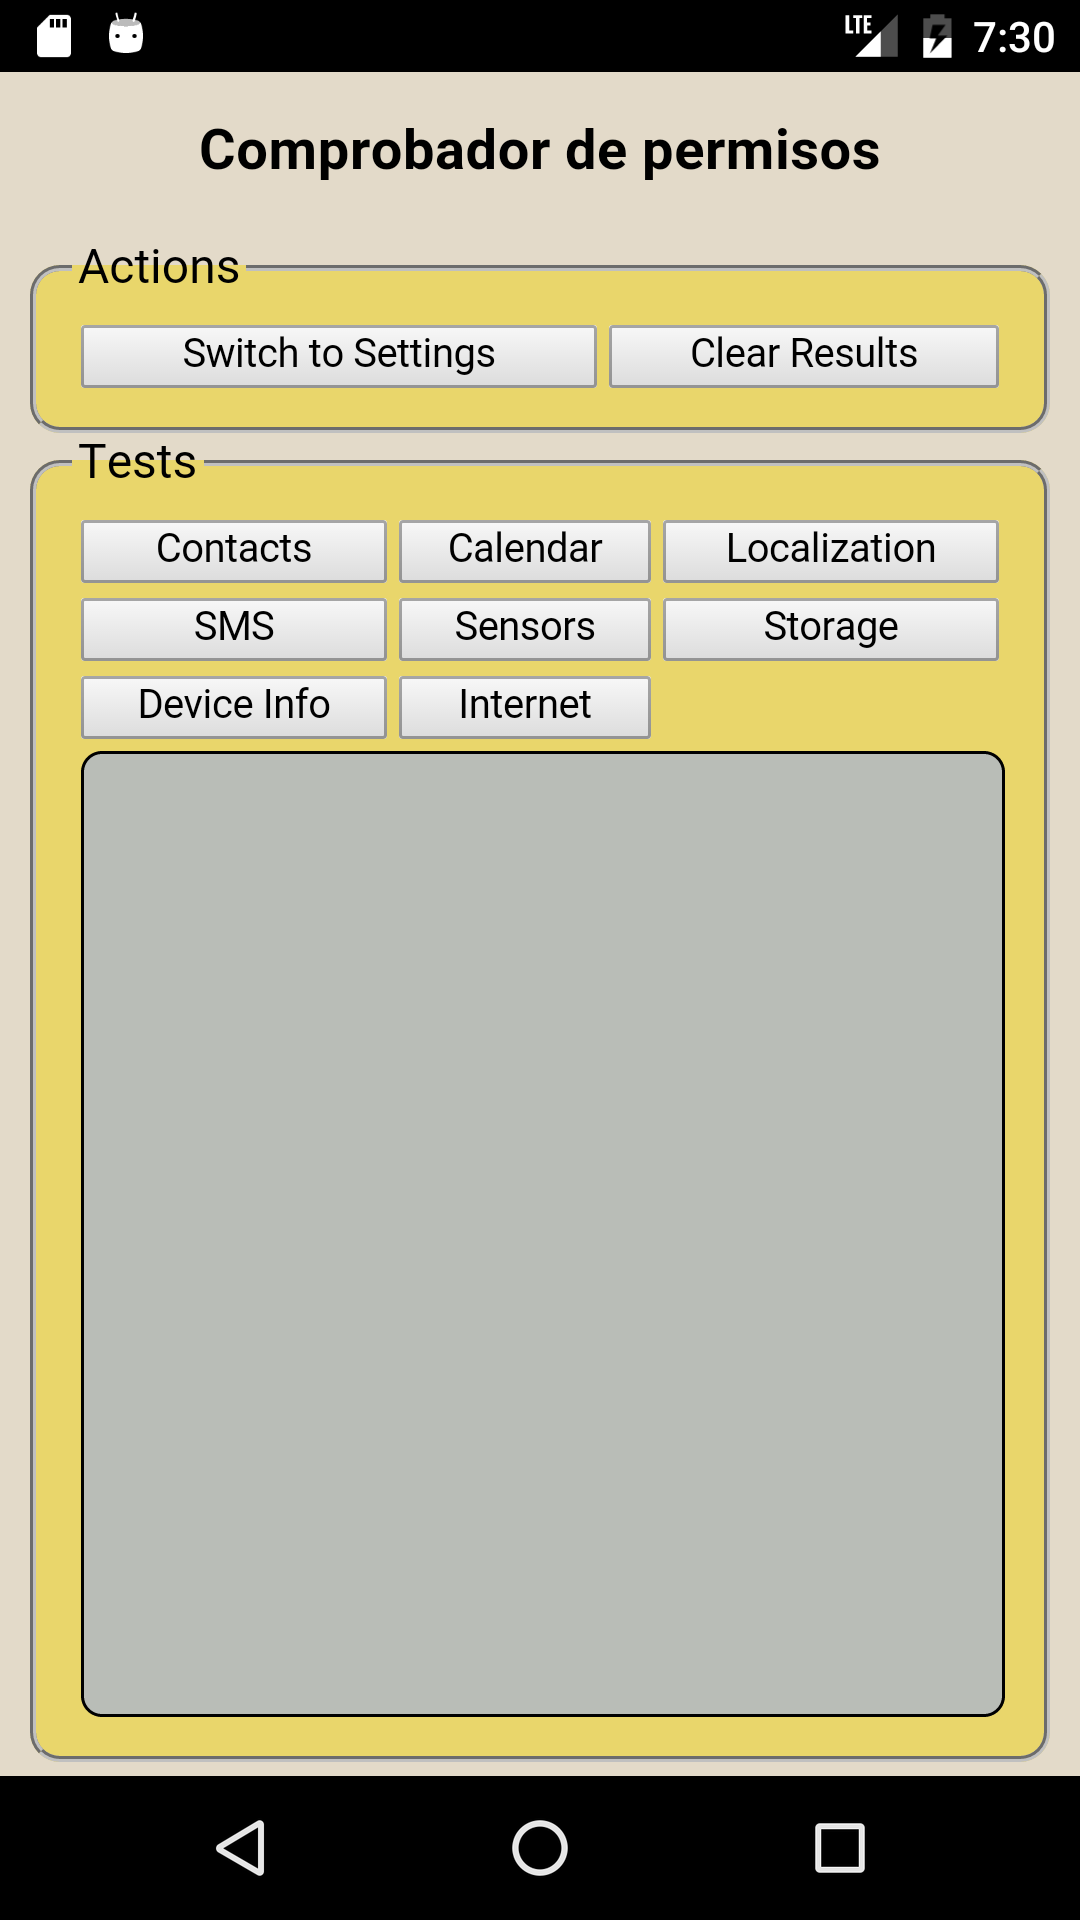
\includegraphics[width=0.75\linewidth]{app_main_view}
	 \caption{Áreas del \textit{framework}.}
	 \label{fig:chapter05:main_view}
    \end{figure}
  \end{column}
  \begin{column}[]{.58\textwidth}
  \begin{block}{}
El \textit{framework} es \alert{una aplicación móvil híbrida} \pause \structure{desarrollada con Apache Cordova} \pause y está compuesto por varios tests.
   \end{block}\pause
   \begin{block}{}
Se utilizaron los emuladores oficiales para testear el \emph{framework} propuesto.
    \end{block}
  \end{column}
 \end{columns}
\end{frame}
\begin{frame}
 \frametitle{Hacia un Framework para la Comparación de Permisos}
 \begin{columns}
  \begin{column}[]{.5\textwidth}
   Utilizando \emph{framework} se pueden testear:
   \begin{itemize}
	\item Contactos
	\item Calendario
	\item Geolocalización
	\item SMS\structure *
	\item Sensores
	\item Almacenamiento
	\item Información del dispositivo
	\item Acceso a Internet
   \end{itemize}
  \end{column}
  \pause
  \begin{column}[]{.5\textwidth}
   Sin embargo, no se pueden testear:
   \begin{itemize}
    \item \alert {WIFI}
    \item \alert {Bluetooth}
    \item \alert {NFC}
    \item \alert {Conexiones USB}
    \item \alert {Micrófono}
    \item \alert {Cámara}
   \end{itemize}
  \end{column}
 \end{columns}
\end{frame}
\begin{frame}
 \frametitle{Hacia un Framework para la Comparación de Permisos}
Por ejemplo:
\begin{figure}[hbp]
    \centering
    \begin{subfigure}{0.28\linewidth}
        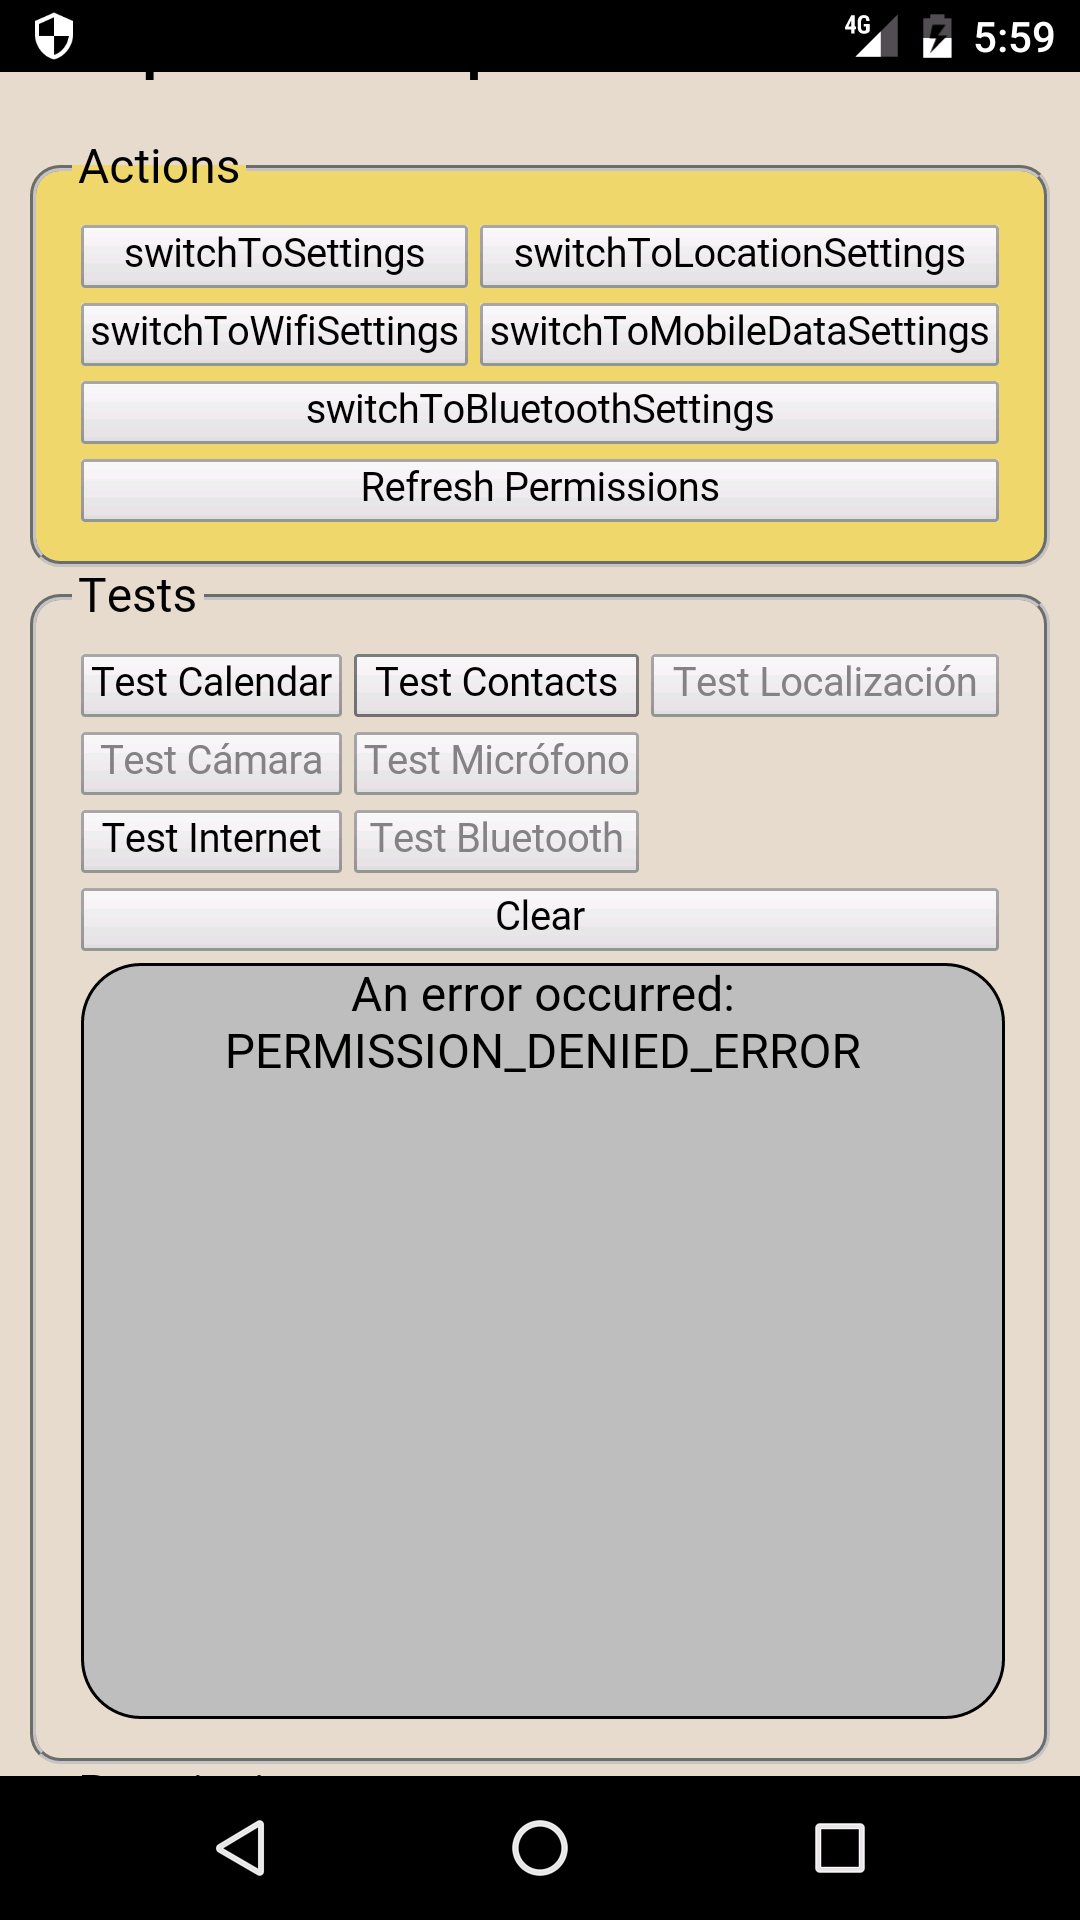
\includegraphics[width=\linewidth]{without_contact}
        \caption{Mensaje de Error.}
    \end{subfigure}
    \begin{subfigure}{0.28\linewidth}
        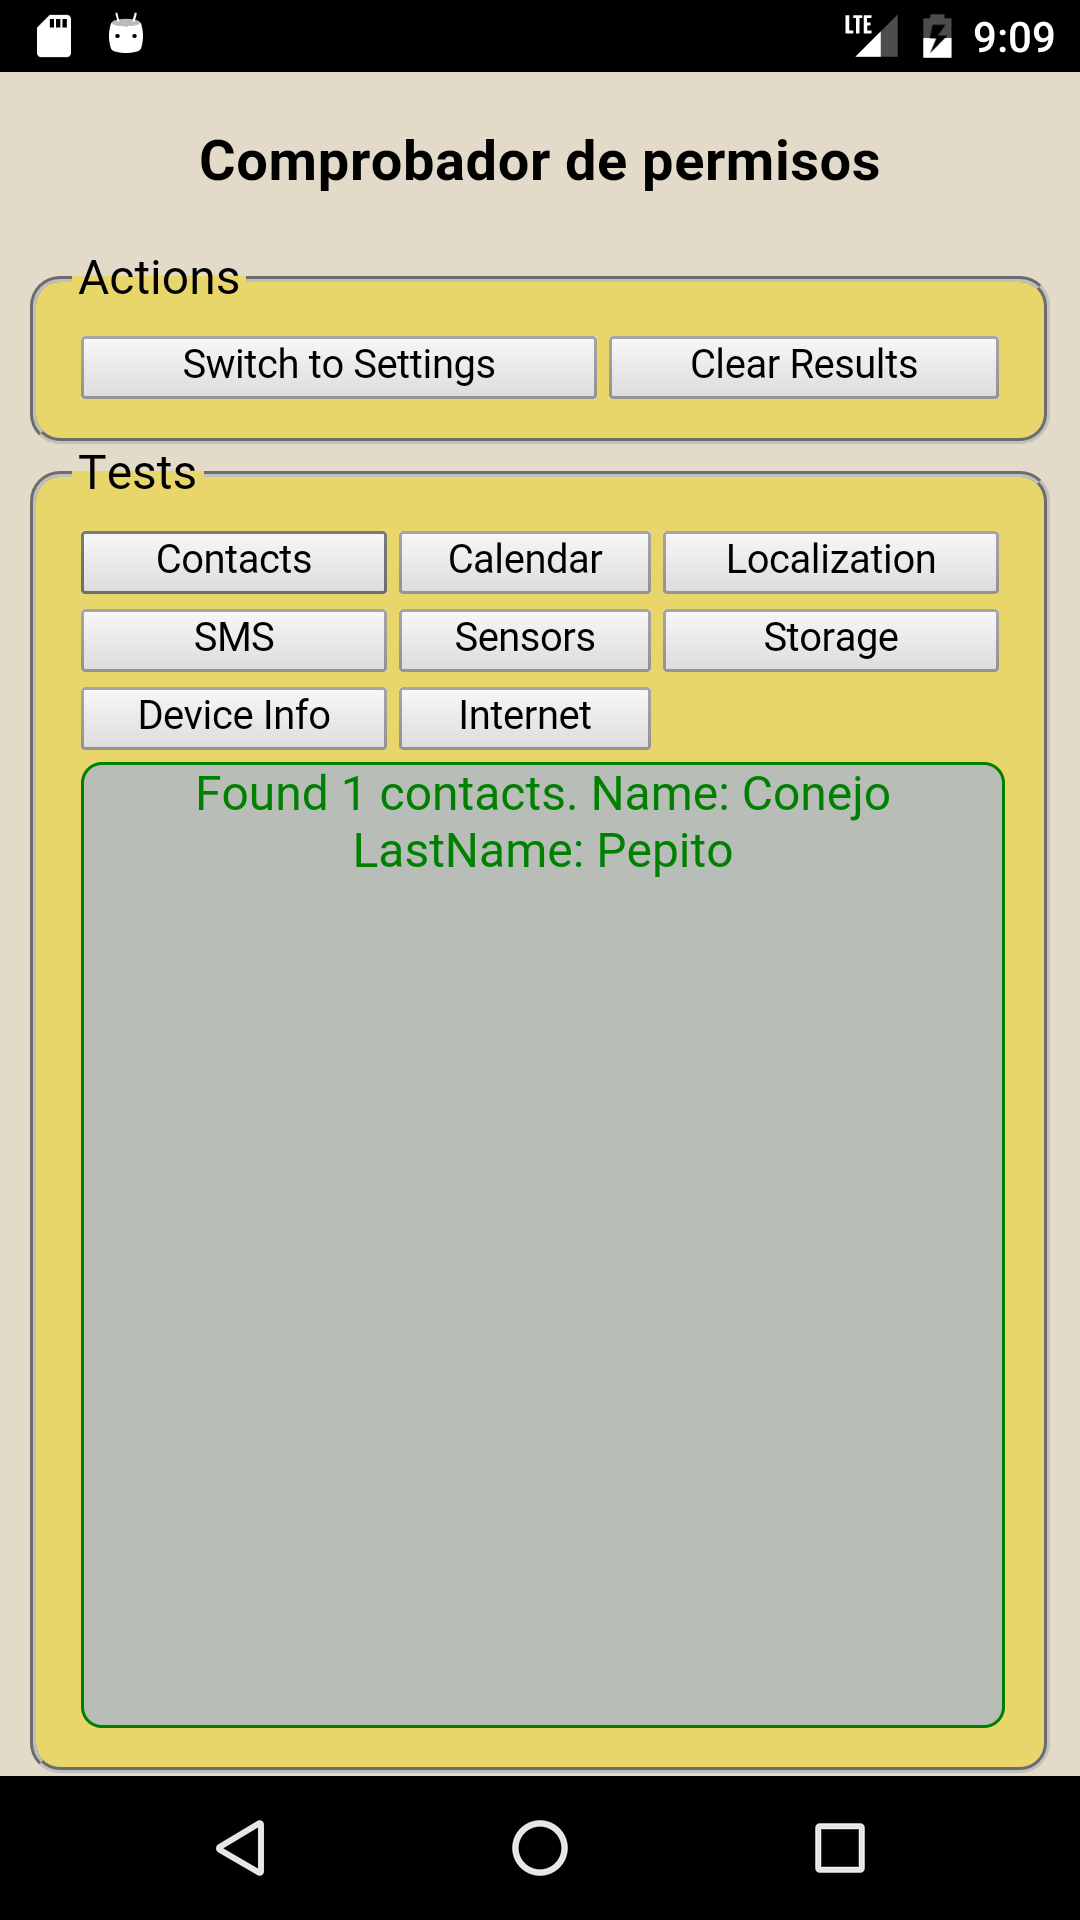
\includegraphics[width=\linewidth]{with_contact}
                \caption{Mensaje exitoso.}
     \end{subfigure}
	\begin{subfigure}{.42\linewidth}
	\begin{algorithm}[H]
	\algsetup{linenosize=\small}
    \scriptsize
	\begin{algorithmic}[1]
		\STATE Se imprimen por consola todos los contactos.
		\STATE Se crea un nuevo contacto.
		\STATE Se vuelven a imprimir por consola \\todos los contactos.
	\end{algorithmic}
	\caption{\centering Test de Contactos}
   \end{algorithm}
   \begin{block}{}\small
    {Es necesario tener el permiso \texttt{Contacto}, tanto para Android como para iOS.}
   \end{block}
   \begin{block}{}\small
 {Se utilizó el \textit{plugin} \texttt{cordova-plugin-contacts} \\(v. 2.3.1).}
   \end{block}
   \end{subfigure}
    \end{figure}
\end{frame}
\begin{frame}
Se pueden clasificar los componentes según \emph{requieran autorización del usuario para utilizarlos}:\pause
  \begin{table}[H]
    \centering
    \begin{small}
	\begin{tabular}{c c c c}
		\hline
		\multicolumn{4}{c}{\emph{\textbf{Permisos}}} \\
		\emph{Clase A} 	& \emph{Clase B}	 & \emph{Clase C}    & \emph{Clase D}\\ \hline \hline
    Contactos    & -    & -    & -\\
    Calendario    & -    & -    & -\\
    Geolocalización    & -    & -    & -\\
    -    & SMS & -    & -\\
    -    & Almacenamiento    & -    & -\\
    -    & -    & -    & Sensores\\
    -    & -    & -    & Información del dispositivo\\
    -    & -    & -    & Acceso a Internet\\ \hline
	\end{tabular}
    \caption{Clasificación de componentes.}
	\end{small}
  \end{table}\pause
  \begin{block}{}\centering
    {Dichas clases mutuamente excluyentes.}  
  \end{block}
\end{frame}